\documentclass[border=4pt]{standalone}
\usepackage{amsmath,amssymb,amsfonts}
\usepackage{xcolor,colortbl,array,booktabs,multirow}
\usepackage{tikz}
\usepackage{pgfplots}
\pgfplotsset{compat=1.16}
\usetikzlibrary{arrows, automata, backgrounds, calendar, chains, decorations,
    matrix, mindmap, patterns, petri, positioning, shadows, shapes.geometric,
    trees, shapes, decorations.pathreplacing, calc, tikzmark, arrows.meta,
    intersections, fit, graphs, quotes, angles, decorations.markings}
\newcommand{\st}{\text{ s.t. }}
\newcommand{\x}{\mathbf{x}}
\renewcommand{\b}{\mathbf{b}}
\renewcommand{\c}{\mathbf{c}}
\newcommand{\A}{\mathbf{A}}
\newcommand{\y}{\mathbf{y}}
\newcommand{\z}{\mathbf{z}}
\newcommand{\R}{\mathbb{R}}
\newcommand{\RR}{\mathbb{R}}
\newcommand{\Z}{\mathbb{Z}}
\newcommand{\ZZ}{\mathbb{Z}}
\newcommand{\npcomplete}{NP-complete}
\providecommand{\true}{\text{TRUE}}
\providecommand{\false}{\text{FALSE}}
\tikzset{vertex/.style={circle,fill=black!25,minimum size=20pt,inner sep=0pt},
    edge/.style={draw,thick,-},weight/.style={font=\small},
    selected vertex/.style={vertex, fill=red!24},
    selected edge/.style={draw,line width=2pt,-,red!50},
    ignored edge/.style={draw,line width=2pt,-,black!20}}
\newcommand{\vect}{\vec}
\providecommand{\ds}{\displaystyle}
\providecommand{\longvect}{\overrightarrow}
\usepackage[normalem]{ulem}
\definecolor{ocre}{RGB}{243,102,25}
\providecommand{\leftB}{\left[}
\providecommand{\rightB}{\right]}
\tikzset{directed/.style={postaction={decorate,decoration={markings,mark=at position .65 with {\arrow{>}}}}},
    directed1/.style={postaction={decorate,decoration={markings,mark=at position .65 with {\arrow{>}}}}}}
\begin{document}
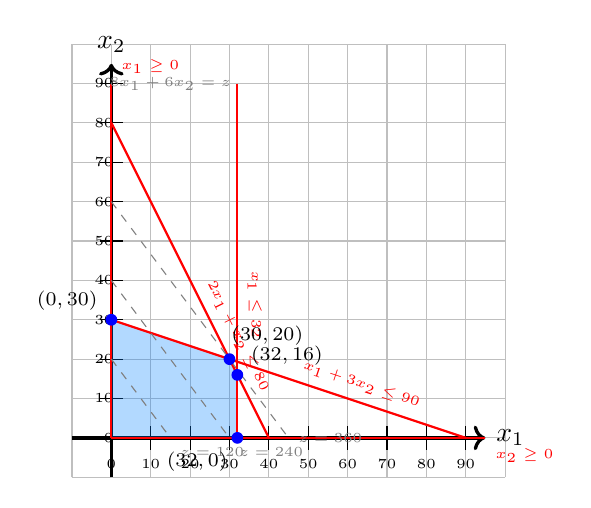
\begin{tikzpicture}[scale=0.05]
    % Grid and axes
    \draw[gray!50, thin, step=10] (-10,-10) grid (100,100);
    \draw[very thick,->] (-10,0) -- (95,0) node[right] {$x_1$};
    \draw[very thick,->] (0,-10) -- (0,95) node[above] {$x_2$};

    % Axis labels
    \foreach \x in {0,10,...,90} \draw (\x,3) -- (\x,-3) node[below] {\tiny\x};
    \foreach \y in {0,10,...,90} \draw (-3,\y) -- (3,\y) node[left] {\tiny\y};

    % Feasible region vertices: (0,0), (0,30), (30,20), (32,16), (32,0)
    \fill[blue!50!cyan,opacity=0.3]
        (0,0) -- (0,30) -- (30,20) -- (32,16) -- (32,0) -- cycle;

    % Constraint lines
    \draw[red,thick] (0,80) --  node[above right, sloped] {\tiny $2x_1 + x_2 \leq 80$}(40,0);
    \draw[red,thick] (0,30) --  node[above right, sloped] {\tiny $x_1 + 3x_2 \leq 90$}(90,0);
    \draw[red,thick] (32,90) --  node[above right, sloped] {\tiny $x_1 \leq 32$}(32,0);
    \draw[red,thick] (0,0) -- (95,0) node[below right] {\tiny $x_2 \geq 0$};
    \draw[red,thick] (0,0) -- (0,90) node[above right] {\tiny $x_1 \geq 0$};

    % Objective function contours (8x1 + 6x2 = z)
    \draw[dashed,gray] (0,120/6) -- (120/8,0) node[below right] {\tiny $z = 120$};
    \draw[dashed,gray] (0,240/6) -- (240/8,0) node[below right] {\tiny $z = 240$};
    \draw[dashed,gray] (0,360/6) -- (360/8,0) node[right] {\tiny $z = 360$};

    % Labels for vertices
    \node[blue] at (0,30) [circle,fill,inner sep=1.5pt]{};
    \node[blue] at (30,20) [circle,fill,inner sep=1.5pt]{};
    \node[blue] at (32,16) [circle,fill,inner sep=1.5pt]{};
    \node[blue] at (32,0) [circle,fill,inner sep=1.5pt]{};

    % Vertex coordinates
    \node[black,anchor=south east] at (-1,30) {\scriptsize $(0,30)$};
    \node[black,anchor=south west] at (28,21) {\scriptsize $(30,20)$};
    \node[black,anchor=south west] at (33,16) {\scriptsize $(32,16)$};
    \node[black,anchor=north east] at (32,-1) {\scriptsize $(32,0)$};

    % Objective function label
    \node[gray] at (15,90) {\tiny $8x_1 + 6x_2 = z$};
\end{tikzpicture}
\end{document}
